\newpage
\section{Kravspecifikation}

\subsection{Indledning}

\subsection{Beskrivelse}
Det endelige system er en sikker meddelelsesplatform, hvori man kan sende og modtage beskeder over et socialt medie, derfor har gruppen tænkt følgende use-case forløb, som et udgangspunkt.

\begin{table}[H]
    \begin{minipage}{.5\textwidth}
        \begin{figure}[H]
            \centering
            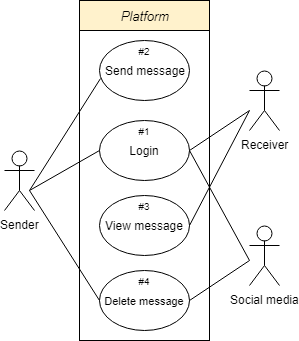
\includegraphics[width=0.85\linewidth]{Projectdoc/Assets/Illustrationer/simple-usecase.png}
            \caption{Usecase diagram}
            \label{fig:usecase}
        \end{figure}
    \end{minipage}
    \begin{minipage}{.5\textwidth}
        \textbf{Herved kan vi definere de givende hovedfunktioner:}
        \begin{itemize}
            \item Brugere skal kunne logge ind i systemet, for betjening.
            \item Systemets sendte beskeder skal deles igennem et socialt medie.
            \item Sendte beskeder skal formaters, for bevarelse af brugerenes sikkerhed.
            \item Systemet skal kunne vise / genindlæse tidligere sendte beskeder.
            \item Brugere skal kunne i systemet kunne slette deres afsendte beskeder.
        \end{itemize}
    \end{minipage}
\end{table}

%Overvejelser\\
%- Anonymt\\
%- Ikke-synlig kommunikation (Skjules blandt uskyldigt indhold på socialt medie)

\section{Metode}